\section{An Example}\label{sec:examples}
To demo the usage of our proposed language constructs in real design and show that the pre-compiler makes work easier and sometimes more interesting, since the programmer can use one statement to express the computation meaning of the circuit structure and gain diverse implementations after compiling it. More examples are attached as appendix.
\subsection{AES}
The AES\cite{AES} algorithm is a symmetric block cipher that processes data block of 128 bits.
Basically, AES operates on a \begin{math} 4 \times 4 \end{math} column-major order matrix (called state) of bytes. The key size used for an AES cipher can be different, and it specifies the number of repetitions of transformation rounds that converts the input, called the plaintext, into the final output, called the ciphertext. 
%%%%%%%%%%%%%%%%%%%%%%%%%%%%%%%%%%%%%%%%%%%%%%%%%%%%
%The numbers of cycles of repetition are as follows:
%\begin{table}[h]
%\centering
%\caption{AES key size}
%\begin{tabular}{|l|l|}
%\hline
%Rounds & Key size \\ \hline
%10 & 128 \\ \hline
%12 & 192 \\ \hline
%14 & 256 \\ \hline
%\end{tabular}
%\vspace{2ex}
%\label{tab:mf}
%\end{table}
%%%%%%%%%%%%%%%%%%%%%%%%%%%%%%%%%%%%%%%%%%%%%%%%%%%%%%
In this example, we take key size as 128-bit. Accordingly it repeats 10 times of the following four steps, in each round.
\begin{itemize}
  \item AddRoundkey(A.R.) - Fig \ref{fig-addroundkey}. Do $\oplus$ operation with $key$.
  \item SubBytes(S.B.) - Fig \ref{fig-subbytes}. Each byte is replaced with its entry in a fixed 8-bit 
        lookup table,
  \item ShiftRows(S.R) - Fig\ref{fig-shiftrows}.Each row of the state are shifted cyclically to the 
        left.
  \item MixColumns(M.C.) - Fig \ref{fig-mixcolumns}. Each column of the state is multiplied with a fixed polynomial 
        $c(x) = 0x03\cdot x^3 + x^2 + x + 0x02$.
\end{itemize}
%
%
%
\begin{figure}
  \centering
  \begin{minipage}[t]{0.4\linewidth}
     \centering
     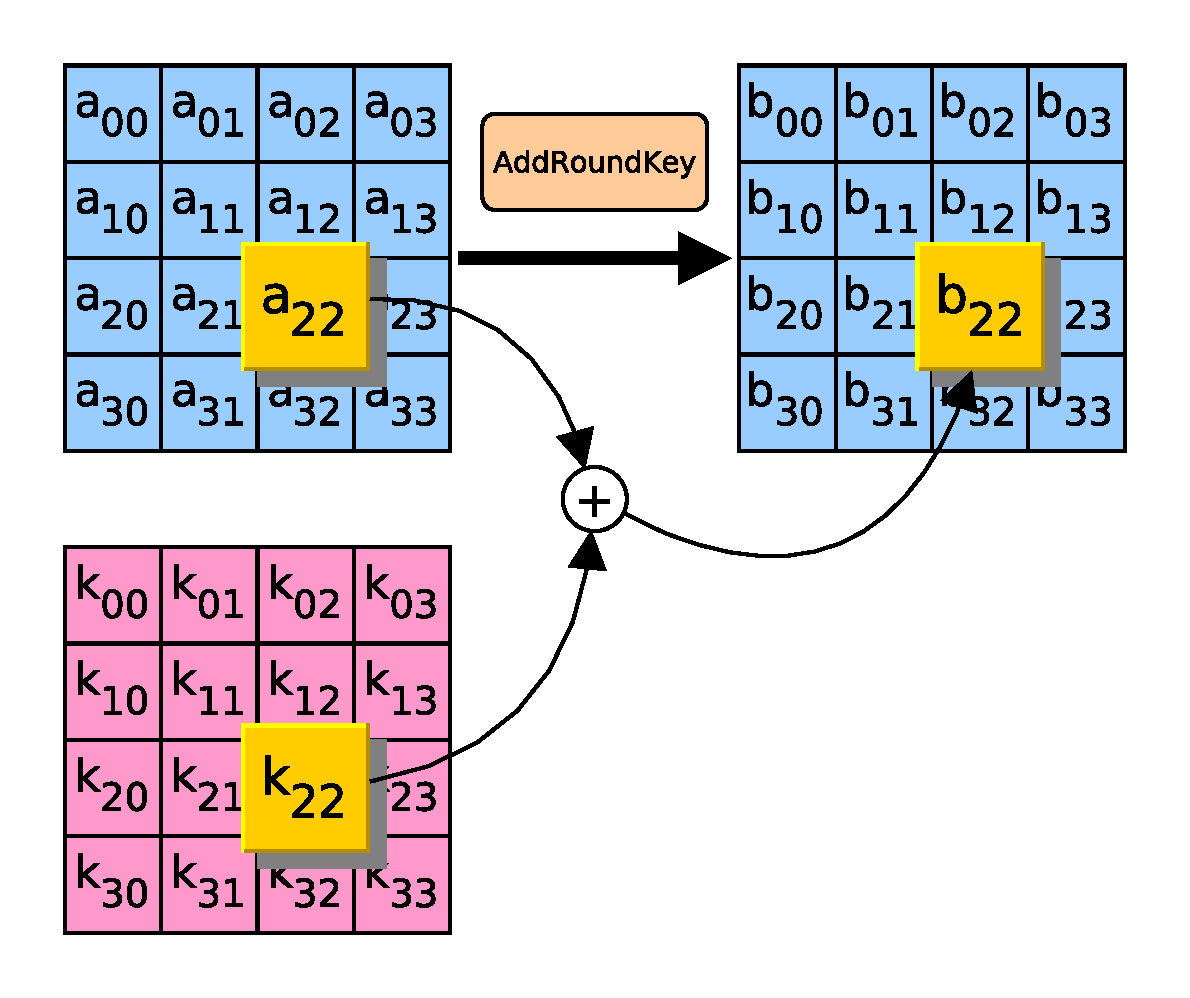
\epsfig{file=addroundkey.eps,width=0.9\columnwidth}
     \caption{A.R.}
     \label{fig-addroundkey}
  \end{minipage}
  \begin{minipage}[t]{0.4\linewidth}
     \centering
     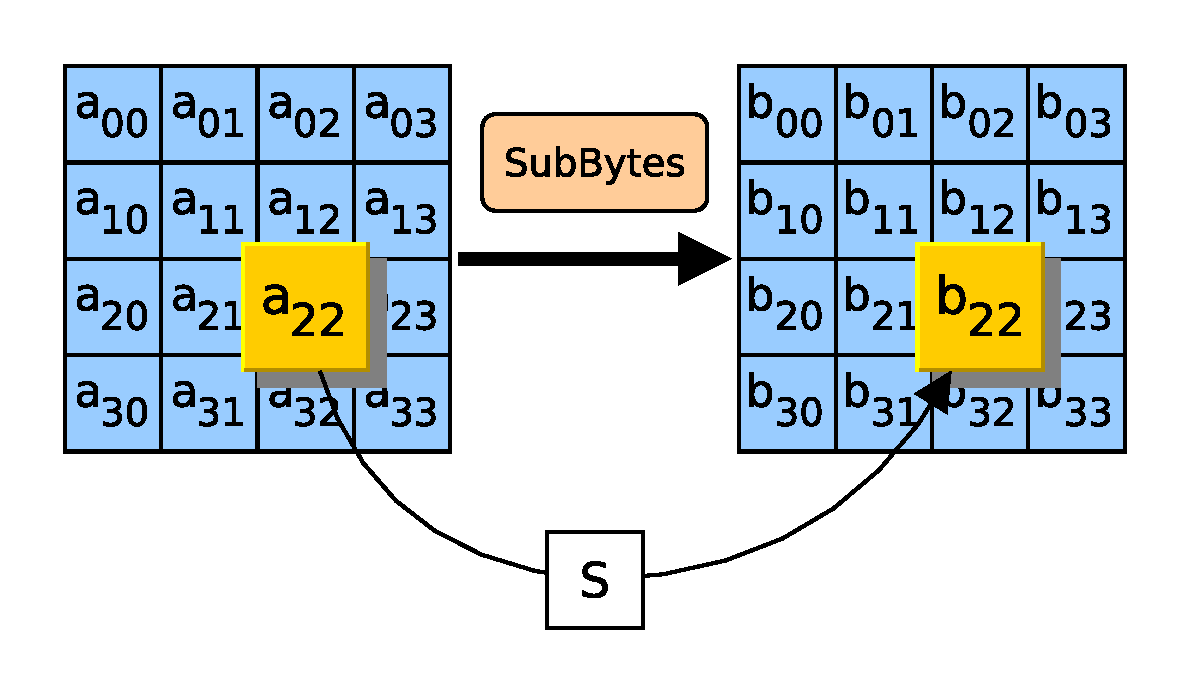
\epsfig{file=subbytes.eps,width=0.9\columnwidth}
     \caption{S.B.}
     \label{fig-subbytes}
  \end{minipage}
  \begin{minipage}[t]{0.4\linewidth}
     \centering
     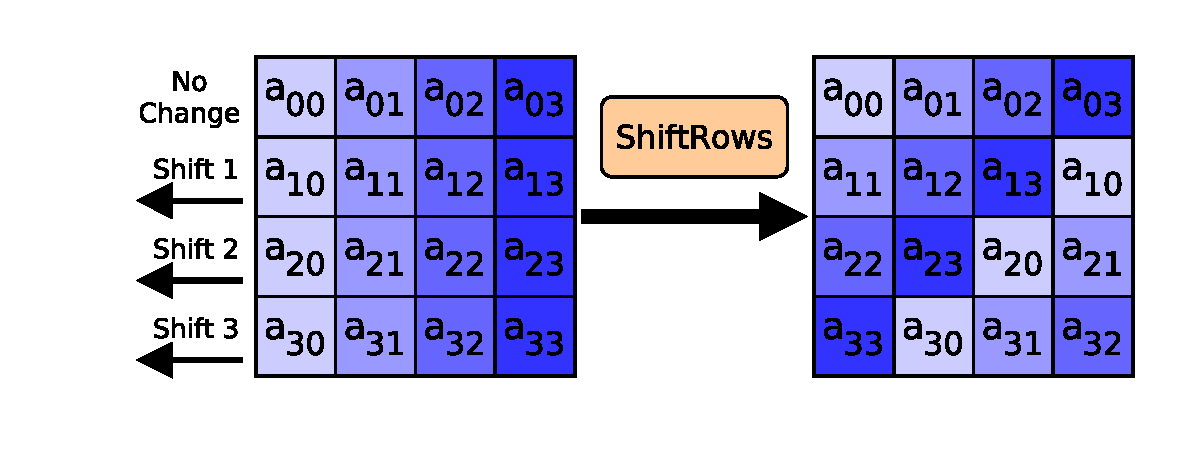
\epsfig{file=shiftrows.eps,width=0.9\columnwidth}
     \caption{S.R.}
     \label{fig-shiftrows}
  \end{minipage}
  \begin{minipage}[t]{0.4\linewidth}
     \centering
     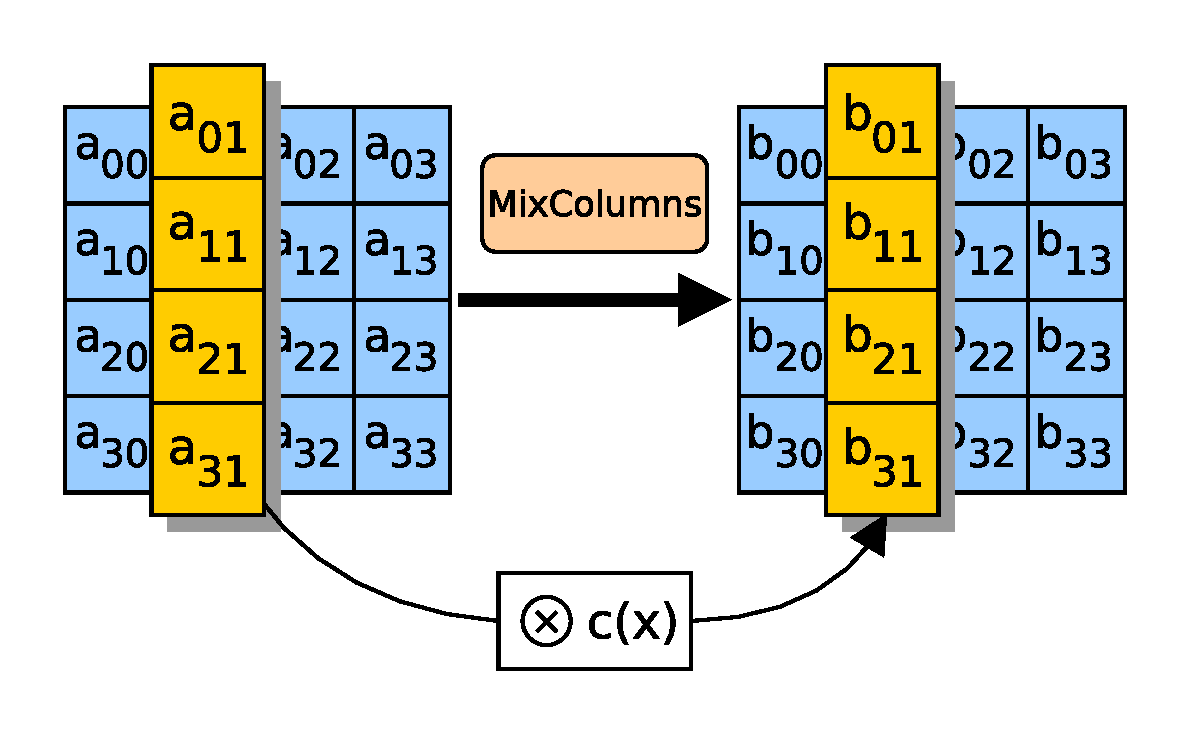
\epsfig{file=mixcolumns.eps,width=0.9\columnwidth}
     \caption{M.C.}
     \label{fig-mixcolumns}
  \end{minipage}
\end{figure}
\subsubsection{Implementatin of AES}
Fig \ref{fig-aesdatapath} shows the dataflow of AES with 128-bit key. We should be aware of that the size of input text is 128-bit, however SubBytes operation gets 8-bit data flows into the S-box each time. So, there comes different configurations of the S-box number. For example, we can use only 1 S-box and do 16 times of SubBytes operations, or use 4 S-box and do just 4 times of SubBytes operations. Same configurations were found in the MixColumns operation.
\begin{figure}[hbpt]
  \centering
  %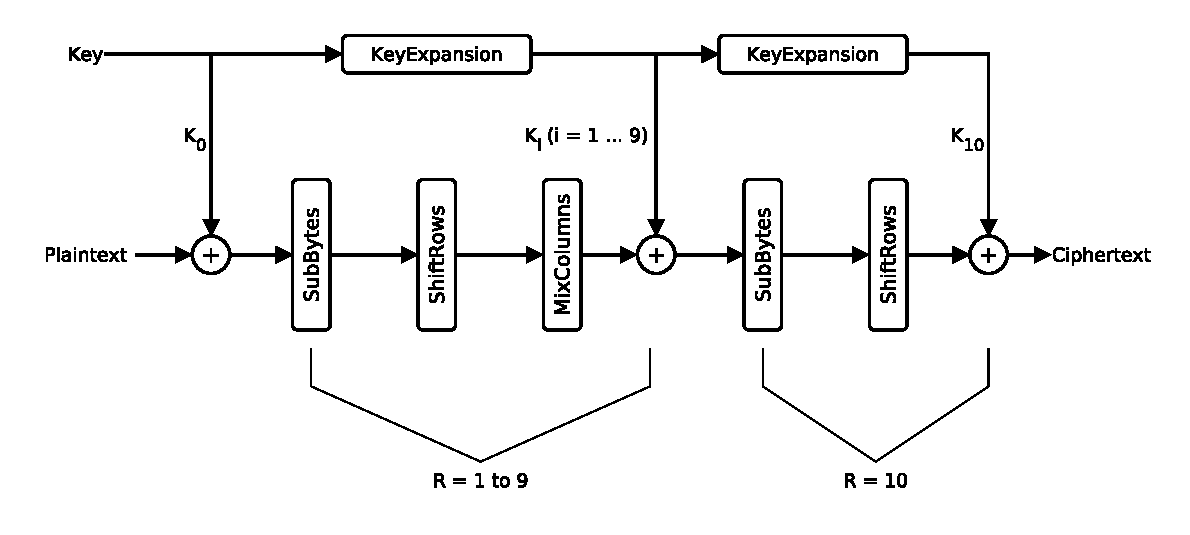
\includegraphics[width=0.1\columnwidth]{DataPathForAES}
  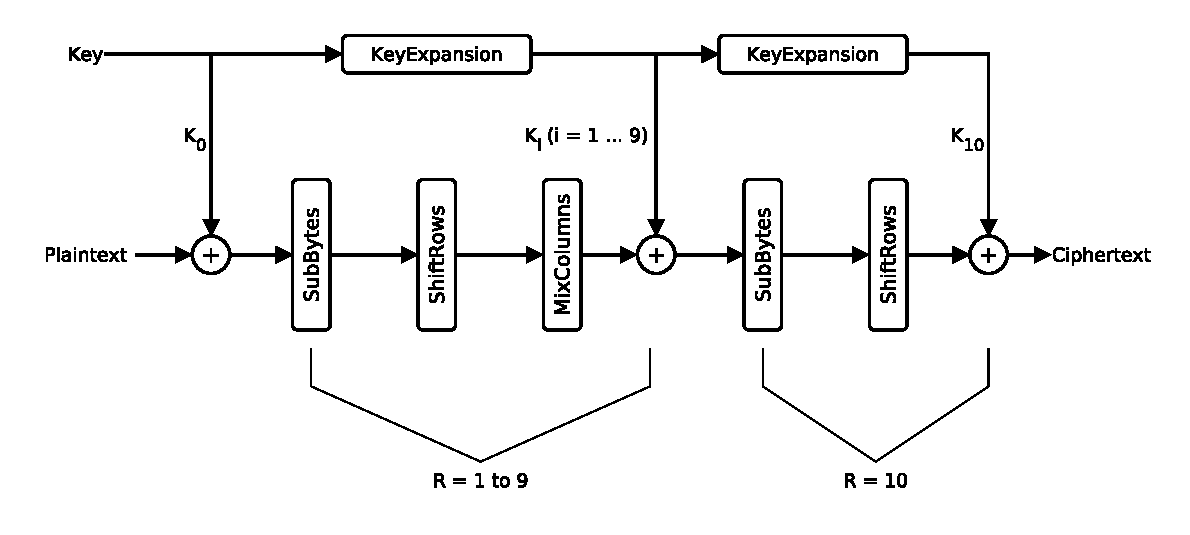
\epsfig{file=DataPathForAES.eps,width=\columnwidth}
  \caption{AES Data Flow}
  \label{fig-aesdatapath}
\end{figure}
\begin{Verbatim}[commandchars=\\\{\}]
always @(posedge clk)
begin   
  if (lddata_i)data <= data_i;
  else if(addkey_i)data <= data_w;
  \Hlight{else if(subbyte_i)map(sbox,data,128,8);}
  else if(mixcolum_i)map(mix,data,128,32);
  else if(shiftrow_i)data <= data_w[127:120], 
                    ..;
end
\end{Verbatim}
%
Where, $sbox$ and $mix$ are two sub-modules, signals $sbox\_i$ and $mixcolumns\_i$ control the invoking of these two sub-modules. Designers don't have to concern the details of the invoke process, such as how $data$ connects with the sub-module, how $data$ flows into sub-module in order. Furthermore, designers can choose the number of sub-modules instances during the compiling process. For different configure choice, the compiler modifies the controller to issue correct control signals in each cycle, as know as  module schedule.

If designers want these configurations without SV+ language constructs, they must write different codes. The following code snippets are just the data transfer part, more codes are needed for module instantiation and $sbox$ input selection.
\begin{Verbatim}[commandchars=\\\{\}]
   Using 1 sbox:           Using 2 sbox:
1. \Vlight{if(subbyte_i)begin     |if(subbyte_i) begin}
2. \Vlight{ data[127:120]<=sbox_o;| data[127:120]<=sbox_o1;}
3. \Vlight{end                    | data[119:112]<=sbox_o0;}
4.                        \Vlight{|end}    
\end{Verbatim}
\begin{Verbatim}[commandchars=\\\{\}]
   Using 4 sboxes:           Using 8, 16 sboxes:
1. \Vlight{if(subbyte_i) begin      | .....}
2. \Vlight{ data[127:120]<=sbox_o3;}
3. \Vlight{ data[119:112]<=sbox_o2;}
4. \Vlight{ data[111:104]<=sbox_o1;}
5. \Vlight{ data[103:96]<=sbox_o0;}
6. \Vlight{end}
\end{Verbatim}